\section{Teilaufgabe 6}
\begin{aufgabe}
    Zeichnen Sie jetzt das asymptotische und realle Bode-Diagramm vom $P_1(s)$ 
    mit dem Befehl asymp. (Diese Routine ist keine Standard Matlab Routine und 
    kann auf ILIAS gefunden werden).
\end{aufgabe}
\begin{figure}[h!]
    \centering
    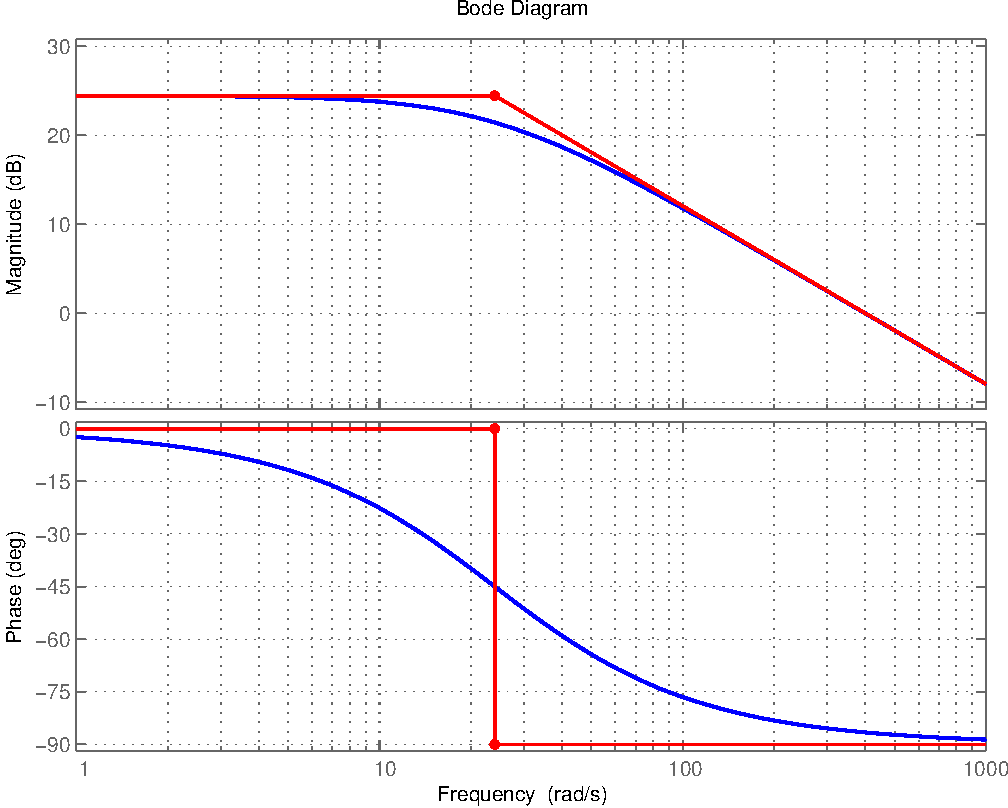
\includegraphics[width=0.6\textwidth]{06/asymp_plot.pdf}
    \caption{Bodediagramm}
    \label{fig:06plot}
\end{figure}
